\documentclass[]{elsarticle} %review=doublespace preprint=single 5p=2 column
%%% Begin My package additions %%%%%%%%%%%%%%%%%%%
\usepackage[hyphens]{url}
\usepackage{lineno} % add
\providecommand{\tightlist}{%
  \setlength{\itemsep}{0pt}\setlength{\parskip}{0pt}}

\bibliographystyle{elsarticle-harv}
\biboptions{sort&compress} % For natbib
\usepackage{graphicx}
\usepackage{booktabs} % book-quality tables
%% Redefines the elsarticle footer
%\makeatletter
%\def\ps@pprintTitle{%
% \let\@oddhead\@empty
% \let\@evenhead\@empty
% \def\@oddfoot{\it \hfill\today}%
% \let\@evenfoot\@oddfoot}
%\makeatother

% A modified page layout
\textwidth 6.75in
\oddsidemargin -0.15in
\evensidemargin -0.15in
\textheight 9in
\topmargin -0.5in
%%%%%%%%%%%%%%%% end my additions to header

\usepackage[T1]{fontenc}
\usepackage{lmodern}
\usepackage{amssymb,amsmath}
\usepackage{ifxetex,ifluatex}
\usepackage{fixltx2e} % provides \textsubscript
% use upquote if available, for straight quotes in verbatim environments
\IfFileExists{upquote.sty}{\usepackage{upquote}}{}
\ifnum 0\ifxetex 1\fi\ifluatex 1\fi=0 % if pdftex
  \usepackage[utf8]{inputenc}
\else % if luatex or xelatex
  \usepackage{fontspec}
  \ifxetex
    \usepackage{xltxtra,xunicode}
  \fi
  \defaultfontfeatures{Mapping=tex-text,Scale=MatchLowercase}
  \newcommand{\euro}{€}
\fi
% use microtype if available
\IfFileExists{microtype.sty}{\usepackage{microtype}}{}
\usepackage{longtable}
\usepackage{graphicx}
% We will generate all images so they have a width \maxwidth. This means
% that they will get their normal width if they fit onto the page, but
% are scaled down if they would overflow the margins.
\makeatletter
\def\maxwidth{\ifdim\Gin@nat@width>\linewidth\linewidth
\else\Gin@nat@width\fi}
\makeatother
\let\Oldincludegraphics\includegraphics
\renewcommand{\includegraphics}[1]{\Oldincludegraphics[width=\maxwidth]{#1}}
\ifxetex
  \usepackage[setpagesize=false, % page size defined by xetex
              unicode=false, % unicode breaks when used with xetex
              xetex]{hyperref}
\else
  \usepackage[unicode=true]{hyperref}
\fi
\hypersetup{breaklinks=true,
            bookmarks=true,
            pdfauthor={},
            pdftitle={Regional Liquor Sales in Iowa},
            colorlinks=true,
            urlcolor=blue,
            linkcolor=magenta,
            pdfborder={0 0 0}}
\urlstyle{same}  % don't use monospace font for urls
\setlength{\parindent}{0pt}
\setlength{\parskip}{6pt plus 2pt minus 1pt}
\setlength{\emergencystretch}{3em}  % prevent overfull lines
\setcounter{secnumdepth}{0}
% Pandoc toggle for numbering sections (defaults to be off)
\setcounter{secnumdepth}{0}
% Pandoc header


\usepackage[nomarkers]{endfloat}

\begin{document}
\begin{frontmatter}

  \title{Regional Liquor Sales in Iowa}
    \author[CUNY School of Professional Studies]{Christophe Hunt\corref{c1}}
   \ead{christophe.hunt@spsmail.cuny.edu} 
   \cortext[c1]{Author}
    \author[CUNY School of Professional Studies]{Senthil Dhanapal}
   \ead{senthil.dhanapal@spsmail.cuny.edu} 
  
    \author[CUNY School of Professional Studies]{Yadu Chittampalli}
   \ead{yadu.chittampalli@spsmail.cuny.edu} 
  
      \address[CUNY School of Professional Studies]{CUNY School of Professional Studies, Data Analytics, New York, NY}
  
  \begin{abstract}
  This is the abstract.
  
  It consists of two paragraphs
  
  \section{\texorpdfstring{Keywords: \emph{Liquor, Liquor
  Sales.}}{Keywords: Liquor, Liquor Sales.}}\label{keywords-liquor-liquor-sales.}
  \end{abstract}
  
 \end{frontmatter}

\section{Problem}\label{problem}

Liquor sales are highly variable and the objective of this report is to
create a statistical model for the volume sold of liquor in gallons by
region within the state of Iowa. This will help us predict inventory and
assist wholesale distributors to plan for predicted volume of
distribution.

\section{Introduction}\label{introduction}

In February, the Distilled Spirits Council (DISCUS), announced that
spirits had an estimated retail sales of nearly \$72 billion in 2015.
Additionally, DISCUS credits the continuous growth of the distilled
spirits industry to several key factors - continuous fascination with
American Whiskeys in the United States and abroad, innovations in
flavors, permutation across all spirits categories leading to consumer
interest, improved regulatory and tax environment resulting in expanded
market access and a relatively low number of state tax threats, and the
growth of small distillers, which expanded grassroots and overall
interest in the spirits category Del Buono (2016).

This establishes that spirit sales in the Unites States is a valuable
market worth exploring for a more detailed and statistical understanding
of sales and volume. We hope to more thoroughly understand what impact
regional and season impacts might have on liquor sales. We will limit
the analysis to Iowa which has also reported sales at a record pace
during the last half of 2000 Boshart (2001). While this older
information we do have data up to 2016 to review.

\section{Research Background (Literature
Review)}\label{research-background-literature-review}

Our goal is inventory prediction.

\section{Methodology}\label{methodology}

The initial data set contained many variables and is sufficiently large
as it includes sales by location and is very granular. The size of the
initial data set has every liquor transaction from 2012 to present so it
approaches 2.68 GB. For the purposes of this analysis, to analyze a data
set this large is not feasible. Therefore, we reduced the number of
variables and summarized to a higher level regional aggregate.

We reduced the data set to \texttt{5} independent variables;
\texttt{County}, \texttt{Category\ name}, \texttt{Bottles\ Sold},
\texttt{Sale\ Dollars}, \texttt{Volume\ Sold\ in\ Gallons}, and our
dependent variable of \texttt{Average\ Price\ Per\ Bottle}.

Additionally, we looked into the top 10 liquor categories for each year
by number of bottles sold. In 2015, the top categories were American
Cocktails, Blended Whiskies, Canadian Whiskies, Imported Vodka, Puerto
Rico \& Virgin Islands Rum, Spiced Rum, Straight Bourbon Whiskies,
Tequila, Vodka 80 Proof, and Whiskey Liqueur. Interestingly straight
bourbon appears to have more sales in 2015 than 2014 which coincides
with the literature of strong growing whiskey sales for every whiskey
segment (Anonymous (2016)).

We initially attempted to model for a dependent variable of
\texttt{Volume\ Sold\ in\ Gallons}, however, the distribution of this
variable becomes over-dispersed and negatively skewed when aggregating
the data set to a manageable size and therefore we were unsuccessful in
modeling this variable. Our hope was that if we could model for the
gallons sold by region we could more accurately predict our planned
inventory and anticipate production goals. We then sought to model the
mean price per bottle, by modeling the price per bottle we can make
pricing decisions based on region and the volume we plan to sell.

discuss the key aspects of your problem, data set and regression
model(s). Given that you are working on real-world data, explain at a
high-level your exploratory data analysis, how you prepared the data for
regression modeling, your process for building regression models, and
your model selection.

\section{Experimentation and Results}\label{experimentation-and-results}

\section{Data Acquisition}\label{data-acquisition}

The data set contains the spirits purchase information of Iowa Class
``E'' liquor licensees by product and date of purchase from January 1,
2012 to current. The data set is provided by the Iowa Department of
Commerce, Alcoholic Beverages Division,
\href{https://data.iowa.gov/Economy/Iowa-Liquor-Sales/m3tr-qhgy}{click
here} to view the data set at Data.Iowa.Gov.

As discussed in our methodogly section, the data set is 2.68 GB in total
size and much to large to process with our current techiniques. A
greater understanding of working with data sets of this size with R w

We reviewed the liquor sales by gallons sold per year by Liquor
Category. Initially, we viewed the top 5 Liquor Categories by volume
sold but there were large disparate between years, suggesting that the
top 5 change often and likely due to changing consumer tastes. See as
the same liquor categories appear consistently for in the top 10
category we chose this level for our model.

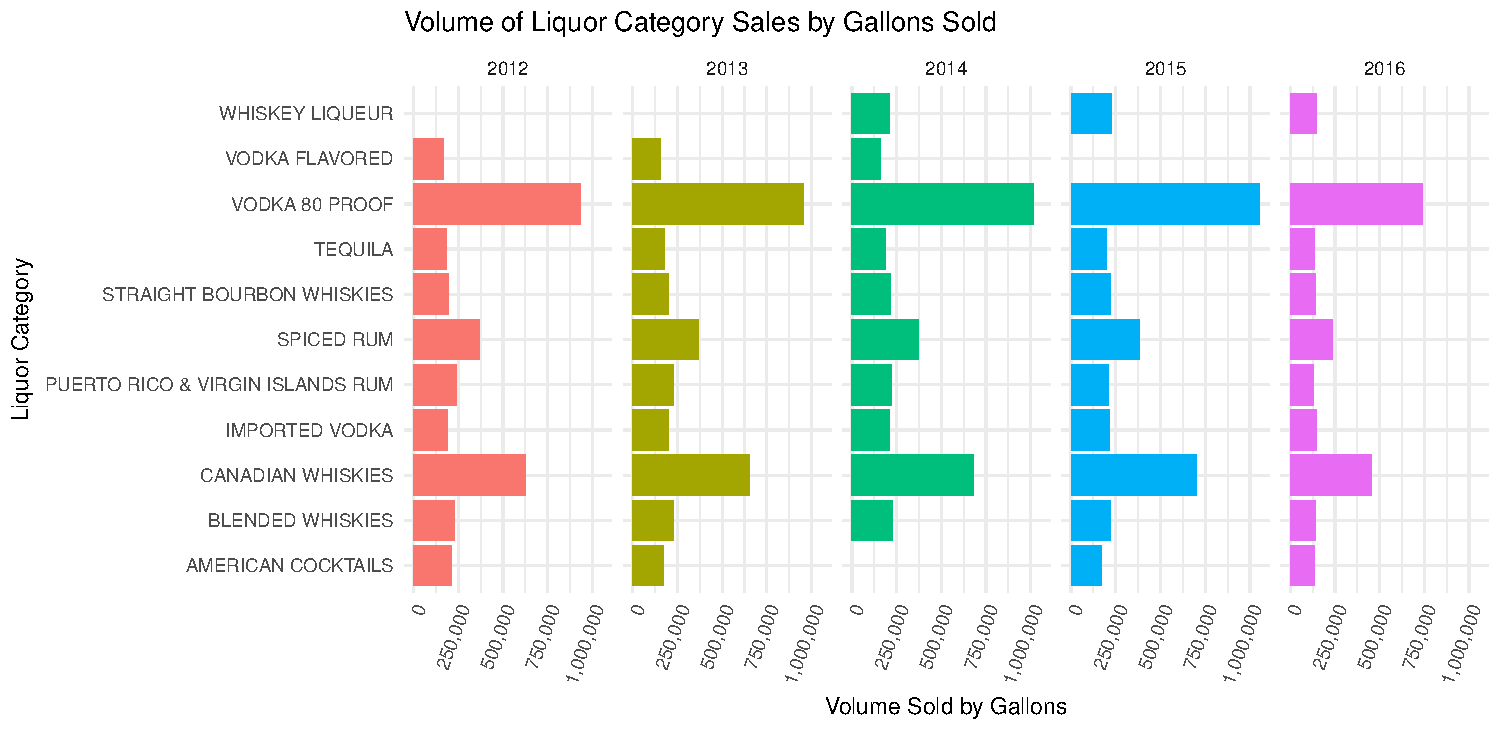
\includegraphics{Final_Project_files/figure-latex/unnamed-chunk-5-1.pdf}

Our first attempt was to use a Poisson regression due to the
over-dispersion created by aggregating the data set. However, the
distribution was far to negatively skewed to fit a poission
distribution. We therefore chose

\subsection{\texorpdfstring{\protect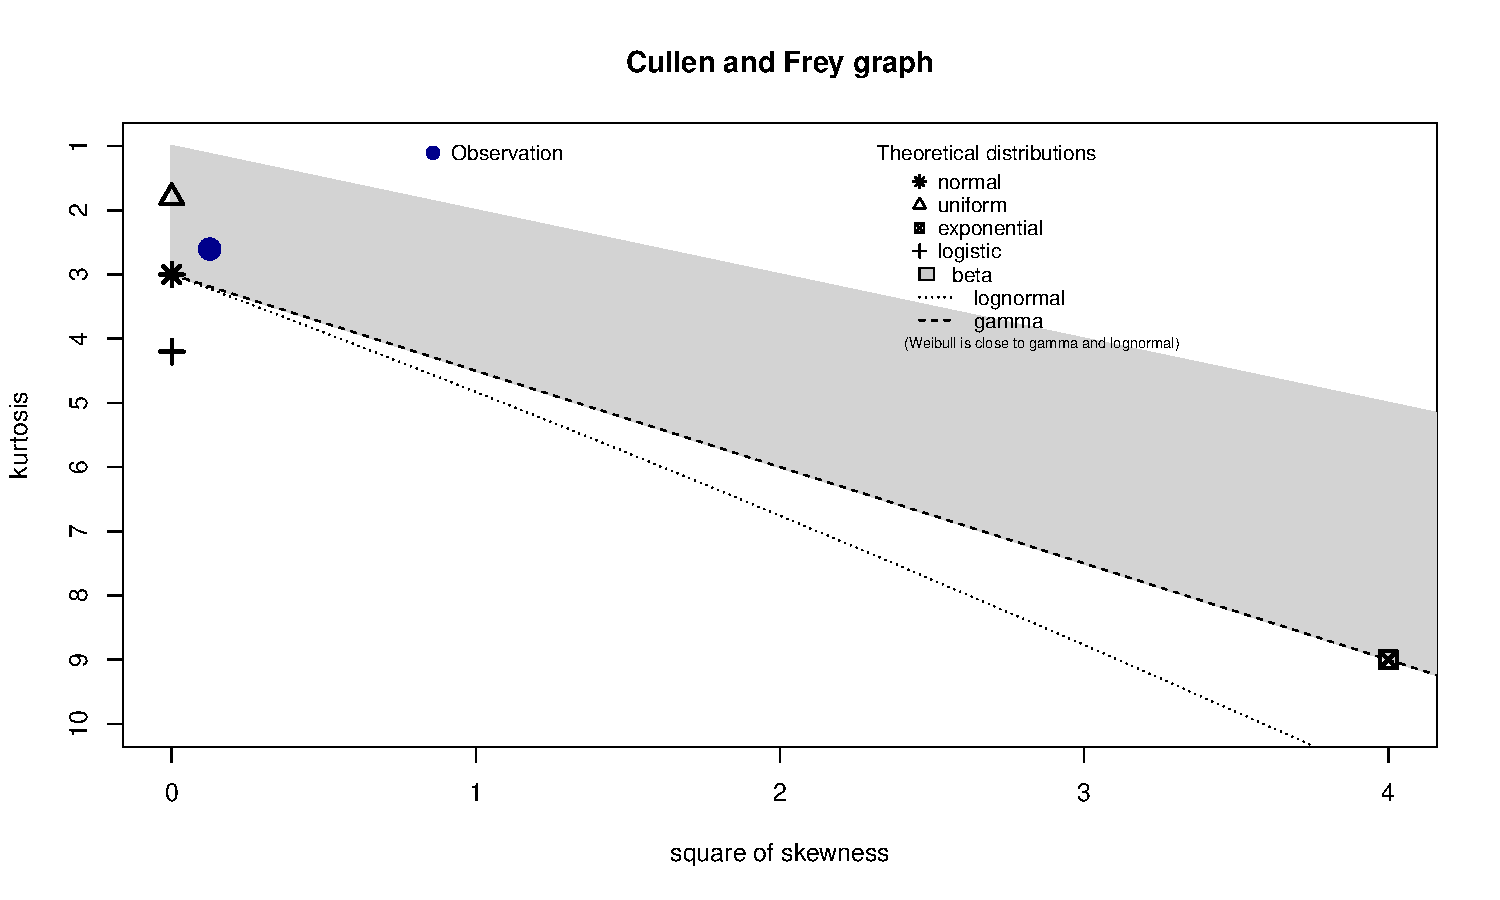
\includegraphics{Final_Project_files/figure-latex/unnamed-chunk-6-1.pdf}}{}}\label{section}

\begin{longtable}[]{@{}cccccccc@{}}
\toprule
min & max & median & mean & sd & skewness & kurtosis &
method\tabularnewline
\midrule
\endhead
6.834324 & 22.80474 & 13.21952 & 13.31821 & 3.604091 & 0.3534382 &
2.604675 & unbiased\tabularnewline
\bottomrule
\end{longtable}

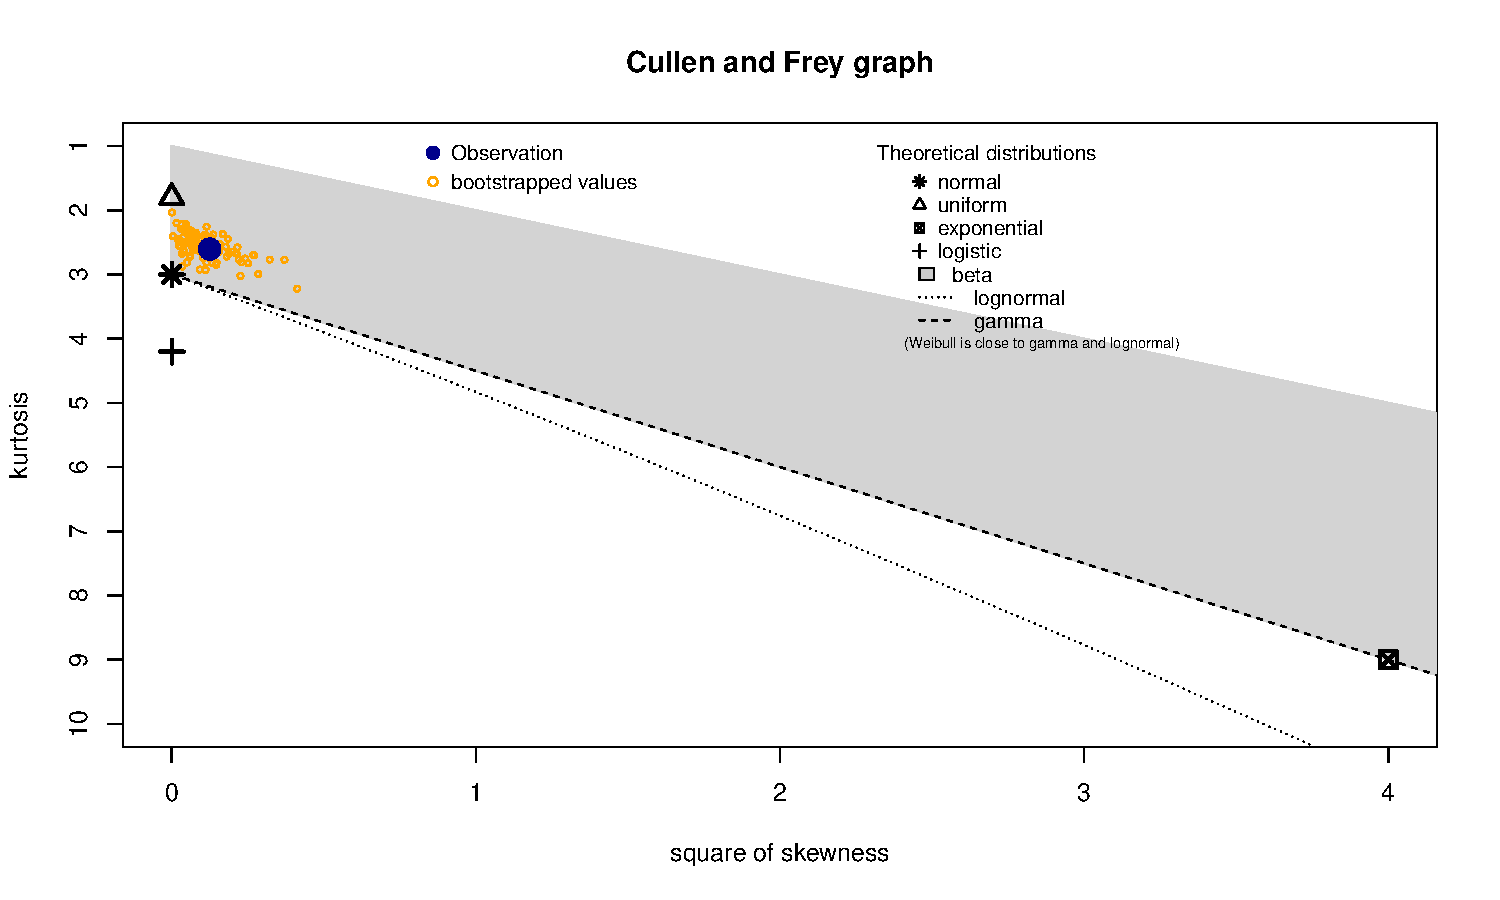
\includegraphics{Final_Project_files/figure-latex/unnamed-chunk-7-1.pdf}

describe the specifics of what you did (data exploration, data
preparation, model building, model selection, model evaluation, etc.),
and what you found out (statistical analyses, interpretation and
discussion of the results, etc.).

\section{Discussion and Conclusions}\label{discussion-and-conclusions}

In another study conducted in 2012 in Idaho, the monthly revenue
generated was examined rather than the yearly revenue generated. The
continued growth was rather owed to the number of weekends a month has
(five instead of four) and to the higher prices in neighboring states.
In Washington, the voters approved an initiative that led the state to
sell its liquor stores and add new distributor and retail fees, making
prices in the neighboring states (Idaho and Oregon) look better. There
were no changes made in marketing or pricing in response to the
regulatory shift in Washington ({\textbf{???}}). Further research into
the proximity of our counties to states and towns with higher prices and
regulation may provide more insight into sales and volume of liquor
sold. Additionally, reviewing the data by identifying months that has 5
weekends instead of four could provide further insights.

conclude your findings, limitations, and suggest areas for future work.

\newpage

\section{Appendices}\label{appendices}

\section{Supplemental tables and/or
figures.}\label{supplemental-tables-andor-figures.}

\section{Session Info}\label{session-info}

\begin{itemize}\raggedright
  \item R version 3.3.2 (2016-10-31), \verb|x86_64-w64-mingw32|
  \item Locale: \verb|LC_COLLATE=English_United States.1252|, \verb|LC_CTYPE=English_United States.1252|, \verb|LC_MONETARY=English_United States.1252|, \verb|LC_NUMERIC=C|, \verb|LC_TIME=English_United States.1252|
  \item Base packages: base, datasets, graphics, grDevices,
    methods, stats, utils
  \item Other packages: fitdistrplus~1.0-7, ggplot2~2.2.0,
    logspline~2.1.9, MASS~7.3-45, pacman~0.4.1, pander~0.6.0,
    survival~2.40-1
  \item Loaded via a namespace (and not attached): assertthat~0.1,
    backports~1.0.4, colorspace~1.3-1, digest~0.6.10,
    evaluate~0.10, grid~3.3.2, gtable~0.2.0, htmltools~0.3.5,
    knitr~1.15.1, lattice~0.20-34, lazyeval~0.2.0, magrittr~1.5,
    Matrix~1.2-7.1, munsell~0.4.3, plyr~1.8.4, Rcpp~0.12.8,
    rmarkdown~1.2, rprojroot~1.1, rticles~0.2, scales~0.4.1,
    splines~3.3.2, stringi~1.1.2, stringr~1.1.0, tibble~1.2,
    tools~3.3.2, yaml~2.1.14
\end{itemize}

\section{R statistical programming
code.}\label{r-statistical-programming-code.}

Please see
\href{https://github.com/ChristopheHunt/DATA-621-Group-1/blob/master/Final\%20Project/Final\%20Project.Rmd}{Final
Project.rmd} on GitHub for source code.

https://github.com/ChristopheHunt/DATA-621-Group-1/blob/master/Final\%20Project/Final\%20Project.Rmd

\section*{References}\label{references}
\addcontentsline{toc}{section}{References}

\hypertarget{refs}{}
\hypertarget{ref-SpecialityGrow3}{}
Anonymous. 2016. ``Specialty Products Grow in Wine, Spirits.''
\emph{Beverage Industry} 107(7).

\hypertarget{ref-IowaSetsRecord2}{}
Boshart, Rod. 2001. ``Liquor Sales in Iowa Set Record.'' \emph{Gazette}.

\hypertarget{ref-KeepingSpiritsHigh1}{}
Del Buono, Amanda. 2016. ``Keeping Spirits High.'' \emph{Beverage
Industry} 107.4: 14--16, 18.

\end{document}


